\section{Appendices}

% Code & documentation used for the project e.g. coding developed
% Screenshots of your code and documentation will suffice here
\subsection{Code and documentation}

\subsubsection{Data loading and pre-processing}

\begin{lstlisting}[caption={Passport tags loading},label={lst:data_loading}]
  import os
  import json
  import pandas as pd

  def get(something, fromTag):
    '''
      Returns the value of the predicate or the tag, extrapolated from
      the URI-formatted string.

      Predicate example: http://www.bbc.co.uk/ontologies/creativework/genre
      Value example: http://www.bbc.co.uk/things/1c3b60a9-14eb-484b-a750-9f5b1aeaac31#id
    '''
      return fromTag.get(something, '').split('/')[-1].split('#')[0]

  def should_skip(predicate):
    '''
      Returns True if the Passport tag is not in the allow list
    '''

    # Allow list of predicates to include in the encoding
    return True if predicate not in [
      'about',
      'format',
      'contributor',
      'genre',
      'motivation',
      'editorialTone',
      'narrativeTheme',
      'relevantTo'
    ] else False

  tags_dict = dict({})
  pids_dict = dict({})
  pids_list = []

  # Lists the Passport files collected from UCED
  uced_files = os.listdir('uced')

  ###
  ## Extrapolates the Passport tags per PID
  ###

  for file_name in uced_files:

    # Gets the PID by splitting "urn:bbc:pips:pid:b05sxyhw.json"
    pid = file_name.split(':')[4].split('.')[0]
    pids_list.append(pid)

    # Loads the JSON file
    with open(f'./uced/{file_name}') as json_file:
        passport = json.loads(json_file.read())

    tags = dict({})

    # For each Passport tag
    for tag in passport.get('taggings', []):
      # Extrapolates the tag's name from the URI
      predicate = get('predicate', tag)

      # Checks the allow list
      if should_skip(predicate):
        continue

      # Extrapolates the tag's value from the URI
      value = get('value', tag)

      # Builds a dictionary of predicates containing a list of values related to the current PID
      if predicate in tags:
        tags[predicate].append(value)
      else:
        tags[predicate] = [value] # list

      # Builds a global dictionary of predicates containing all the tag values used for all PIDs.
      # These tag values may be repeated across predicates.
      if predicate in tags_dict:
        tags_dict[predicate].add(value)
      else:
        tags_dict[predicate] = {value} # set

    # Builds the dictionary of PIDs, with the associated predicate tags
    pids_dict[pid] = tags
\end{lstlisting}

\begin{lstlisting}[caption={One-hot encoding of the data in a Pandas DataFrame},label={lst:data_encoding}]
  ###
  ## I need to build a dataframe where the rows are indexed by the PIDs, and the columns indexed by the Passport tags.
  ## To this end, I need to create a multi-index for the columns, where the first level is the tag predicate,
  ## and the second level the tag value. This will allow duplicate of values across predicates, and access to any
  ## given cell by speficying the PID, the predicate and the value, in order for the algorithm to set the value "1"
  ## to signal the PID is tagged.
  ###

  columns = []

  for key in tags_dict.keys():
    columns.extend(pd.MultiIndex.from_product([[key], tags_dict.get(key)]))

  ###
  ## Creates a zero-filled dataframe of type integer with PIDs as row indexes and the Passport predicates and tags
  ## as multi-level column index, as specified earlier.
  ###

  df = pd.DataFrame(0, index=pids_list, columns=pd.MultiIndex.from_tuples(columns), dtype='uint8')

  ###
  ## Sets 1 for each PID and predicate/tag pair (i.e. One-Hot Encoding)
  ###

  for pid in pids_dict.keys():
    for predicate in pids_dict[pid].keys():
      for tag in pids_dict.get(pid).get(predicate):
        df.at[pid, (predicate, tag)] = 1

  ###
  ## Drops the first level of the multi-level column index to flatten the dataframe, now that it is no longer needed.
  ###

  df = df.droplevel(level=0, axis=1)
\end{lstlisting}

\subsubsection{Model training}

\begin{lstlisting}[caption={Dataset splitting},label={lst:data_splitting}]
  import pandas as pd
  from sklearn.model_selection import train_test_split

  data = pd.read_parquet('passport_encoding.parquet')

  X_train, X_test = train_test_split(data, test_size=0.2)
  X_val, X_test = train_test_split(X_test, test_size=0.5)

  assert X_train.shape[0] + X_val.shape[0] + X_test.shape[0] == data.shape[0]
\end{lstlisting}

\begin{lstlisting}[caption={Model training and hyperparameter tuning with Keras and KerasTuner},label={lst:hyperband}]
  import tensorflow as tf
  from tensorflow import keras
  import keras_tuner as kt

  # https://www.tensorflow.org/tutorials/keras/keras_tuner

  input_size = X_train.shape[1]

  # https://keras.io/api/keras_tuner/hyperparameters/
  def build_model(hp: kt.HyperParameters):
    # Parameters Set
    hidden_layers = hp.Choice('hidden_layers', [1, 3])
    embeddings_size = hp.Choice('embeddings_size', [70, 140, 280, 560])
    batch_norm = hp.Boolean('batch_norm')
    dropout = hp.Boolean('dropout')
    learning_rate = hp.Choice('learning_rate', [0.1, 0.01, 0.001])

    activation = 'relu'
    dropout_rate = 0.2

    model = keras.Sequential()
    model.add(keras.layers.InputLayer(input_shape=(input_size,)))

    if hidden_layers == 1:
      model.add(keras.layers.Dense(
        units=embeddings_size,
        activation=activation
      ))
      if batch_norm:
        model.add(keras.layers.BatchNormalization())
      if dropout:
        model.add(keras.layers.Dropout(dropout_rate))

    if hidden_layers == 3:
      model.add(keras.layers.Dense(
        units=embeddings_size * 2,
        activation=activation
      ))
      if batch_norm:
        model.add(keras.layers.BatchNormalization())
      if dropout:
        model.add(keras.layers.Dropout(dropout_rate))

      model.add(keras.layers.Dense(
        units=embeddings_size,
        activation=activation
      ))
      if batch_norm:
        model.add(keras.layers.BatchNormalization())
      if dropout:
        model.add(keras.layers.Dropout(dropout_rate))

      model.add(keras.layers.Dense(
        units=embeddings_size * 2,
        activation=activation
      ))
      if batch_norm:
        model.add(keras.layers.BatchNormalization())
      if dropout:
        model.add(keras.layers.Dropout(dropout_rate))

    if hidden_layers == 3:
      model.add(keras.layers.Dense(
        units=embeddings_size * 4,
        activation=activation
      ))
      if batch_norm:
        model.add(keras.layers.BatchNormalization())
      if dropout:
        model.add(keras.layers.Dropout(dropout_rate))

      model.add(keras.layers.Dense(
        units=embeddings_size * 2,
        activation=activation
      ))
      if batch_norm:
        model.add(keras.layers.BatchNormalization())
      if dropout:
        model.add(keras.layers.Dropout(dropout_rate))

      model.add(keras.layers.Dense(
        units=embeddings_size,
        activation=activation
      ))
      if batch_norm:
        model.add(keras.layers.BatchNormalization())
      if dropout:
        model.add(keras.layers.Dropout(dropout_rate))

      model.add(keras.layers.Dense(
        units=embeddings_size * 2,
        activation=activation
      ))
      if batch_norm:
        model.add(keras.layers.BatchNormalization())
      if dropout:
        model.add(keras.layers.Dropout(dropout_rate))

      model.add(keras.layers.Dense(
        units=embeddings_size * 4,
        activation=activation
      ))
      if batch_norm:
        model.add(keras.layers.BatchNormalization())
      if dropout:
        model.add(keras.layers.Dropout(dropout_rate))

      model.add(keras.layers.Dense(input_size, activation='sigmoid'))

      model.compile(
          optimizer=keras.optimizers.Adam(learning_rate=learning_rate),
          loss=keras.losses.BinaryCrossentropy()
      )

      return model
\end{lstlisting}

\begin{lstlisting}[caption={Hyperband search and early stopping setup},label={lst:hyperband_search}]
  # https://keras.io/api/keras_tuner/tuners/hyperband/
  tuner = kt.Hyperband(
    hypermodel=build_model,
    objective='val_loss',
    max_epochs=100,
    factor=2
  )

  early_stop = tf.keras.callbacks.EarlyStopping(
    monitor='val_loss',
    mode='min',
    restore_best_weights=True,
    patience=10
  )

  tuner.search(
    X_train,
    X_train,
    epochs=100,
    batch_size=300,
    verbose=1,
    callbacks=[early_stop],
    validation_data=(X_val, X_val)
  )
\end{lstlisting}

\begin{lstlisting}[caption={Best model re-training},label={lst:model_retraining}]
  best_hp = tuner.get_best_hyperparameters()[0]
  model = tuner.hypermodel.build(best_hp)

  history = model.fit(
    X_train,
    X_train,
    epochs=100,
    batch_size=300,
    verbose=1,
    callbacks=[early_stop],
    validation_data=(X_val, X_val)
  )
\end{lstlisting}

\begin{lstlisting}[caption={Binary cross-entropy loss visualisation},label={lst:loss_visualisation}]
  val_loss = history.history['val_loss']
  best_epoch = val_loss.index(min(val_loss)) + 1
  print(f'Best epoch: {best_epoch}')

  import matplotlib.pyplot as plt

  plt.plot(history.history['loss'], label='Training')
  plt.plot(history.history['val_loss'], label='Validation')
  plt.ylabel('Binary Cross Entropy Loss')
  plt.xlabel('Epochs')
  plt.ylim((0, 0.003))
  plt.legend()
  plt.show();
\end{lstlisting}

\subsubsection{Embeddings}

\begin{lstlisting}[caption={Embeddings generation},label={lst:embeddings}]
  from tensorflow.keras import Model

  # Defines Input/Output of the model
  input = autoencoder.input
  output = autoencoder.get_layer(name='code').output

  # Defines the embedding generator model using the encoder part of the trained Autoencoder model
  embedding_generator = Model(name='Embedding_Generator', inputs=input, outputs=output)

  # Generates the embeddings by using the output of the bottleneck layer
  embeddings = embedding_generator.predict(data)
\end{lstlisting}

\subsubsection{Recommendations}

\begin{lstlisting}[caption={Cosine similarity calculation},label={lst:cosine_similarity}]
  import pandas as pd
  from sklearn.metrics.pairwise import cosine_similarity

  # Loads the catalogue
  catalogue = pd.read_parquet('catalogue.parquet')
  # Gets the PIDs of the programmes to recommend (Top-Level Editorial Objects)
  tleo = catalogue.tleo_pid.values
  # Loads the embeddings
  embeddings = pd.read_parquet('560_1_relu.parquet')
  # Gets the TLEOs embeddings
  tleo_embeddings = embeddings[embeddings.index.isin(tleo)]
  # Generates the similarity matrix
  similarity = pd.DataFrame(cosine_similarity(tleo_embeddings), index=tleo_embeddings.index, columns=tleo_embeddings.index)
\end{lstlisting}

% Figures / tables / visualisation as appropriate to the project

\subsection{Figures and tables}

\subsubsection{Passport tags}

\begin{figure}[H]
  \centering
  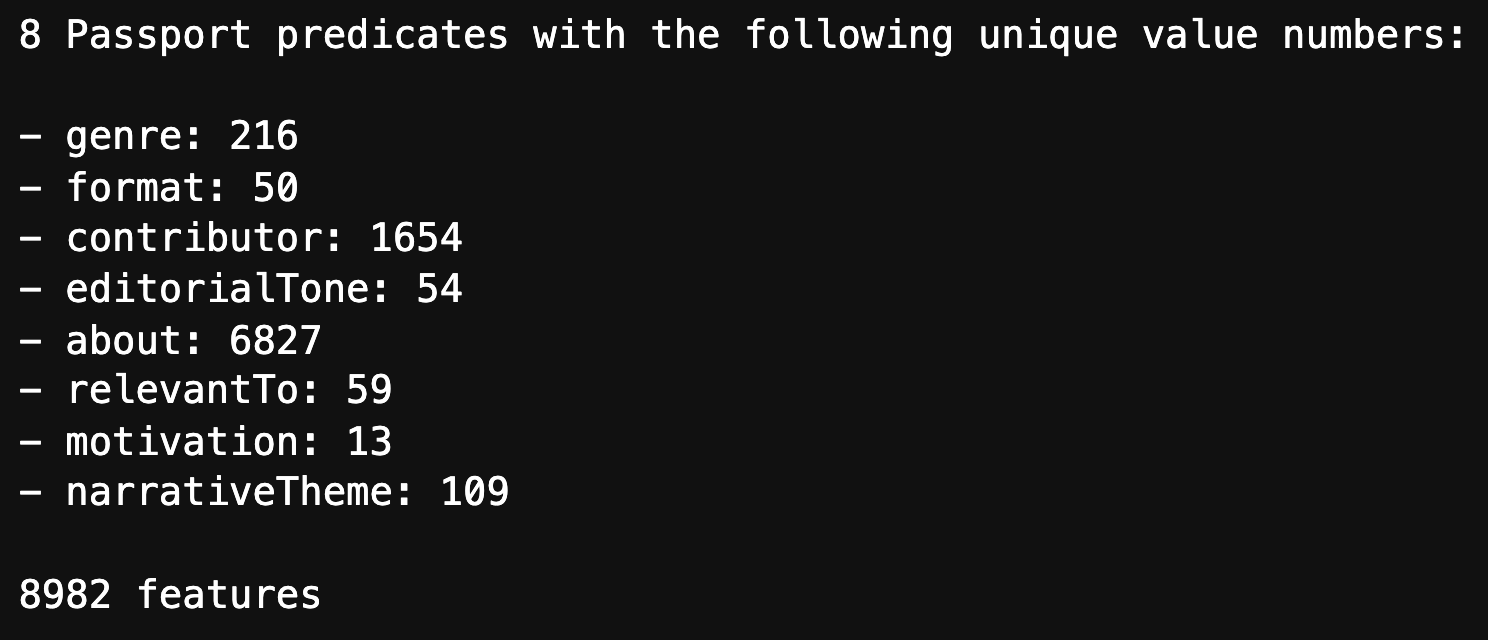
\includegraphics[scale=0.5]{passport_stats}
  \caption{Number of unique value annotations per Passport tag}
  \label{fig:passport_stats}
\end{figure}

\begin{figure}[H]
  \centering
  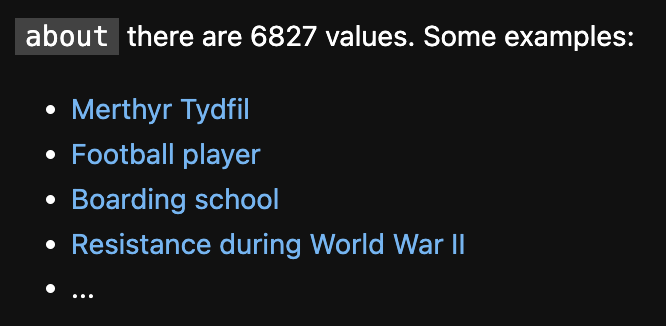
\includegraphics[scale=0.8]{tag_about}
  \caption{The "about" tag}
  \label{fig:tag_about}
\end{figure}

\begin{figure}[H]
  \centering
  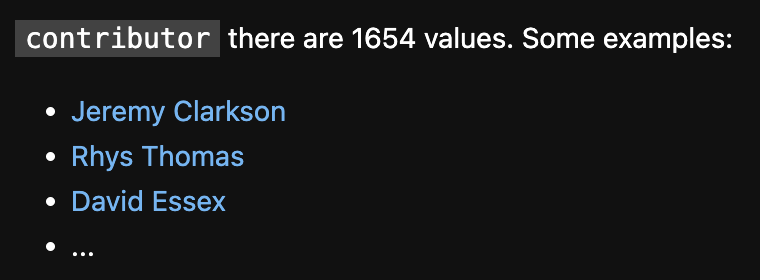
\includegraphics[scale=0.8]{tag_contributor}
  \caption{The "contributor" tag}
  \label{fig:tag_contributor}
\end{figure}

\begin{figure}[H]
  \centering
  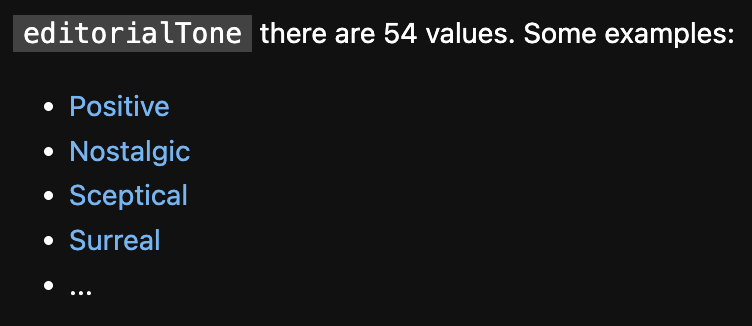
\includegraphics[scale=0.8]{tag_editorialTone}
  \caption{The "editorialTone" tag}
  \label{fig:tag_editorialTone}
\end{figure}

\begin{figure}[H]
  \centering
  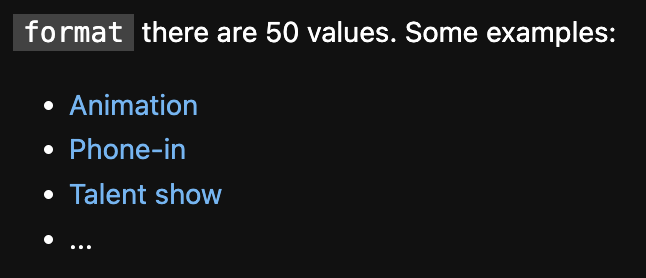
\includegraphics[scale=0.8]{tag_format}
  \caption{The "format" tag}
  \label{fig:tag_format}
\end{figure}

\begin{figure}[H]
  \centering
  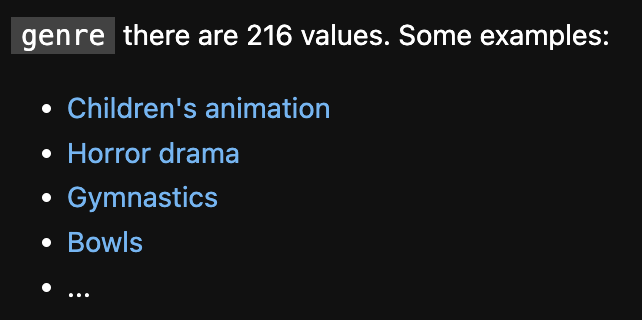
\includegraphics[scale=0.8]{tag_genre}
  \caption{The "genre" tag}
  \label{fig:tag_genre}
\end{figure}

\begin{figure}[H]
  \centering
  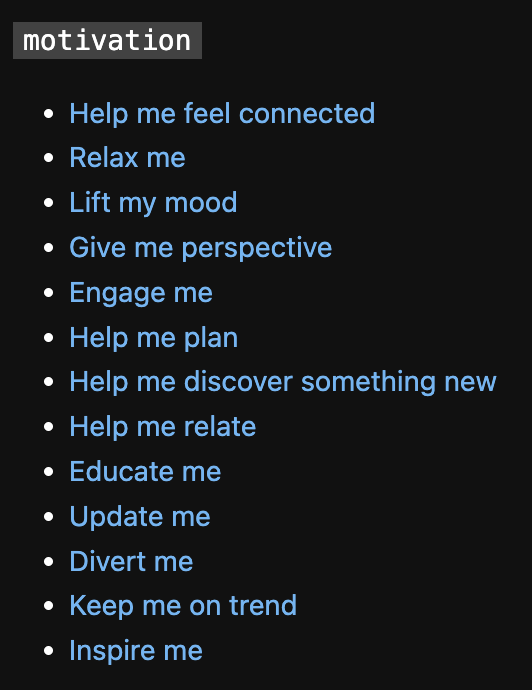
\includegraphics[scale=0.8]{tag_motivation}
  \caption{The "motivation" tag}
  \label{fig:tag_motivation}
\end{figure}

\begin{figure}[H]
  \centering
  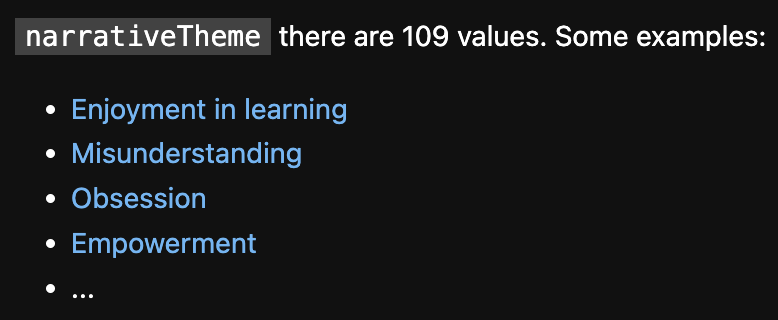
\includegraphics[scale=0.8]{tag_narrativeTheme}
  \caption{The "narrativeTheme" tag}
  \label{fig:tag_narrativeTheme}
\end{figure}

\begin{figure}[H]
  \centering
  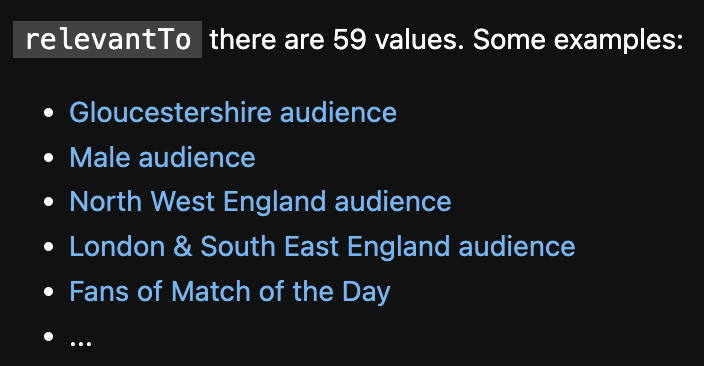
\includegraphics[scale=0.8]{tag_relevantTo}
  \caption{The "relevantTo" tag}
  \label{fig:tag_relevantTo}
\end{figure}

\subsubsection{Catalogue analysis}

The following line plots visualise the daily time-series statistics of the BBC iPlayer catalogue used for training.
New programmes are added to the catalogue, and unavailable ones are removed hourly.
These updates change the size and tag composition of the catalogue and need to be monitored for data drift detection,
retraining the model when big spikes occur.

\begin{figure}[H]
  \centering
  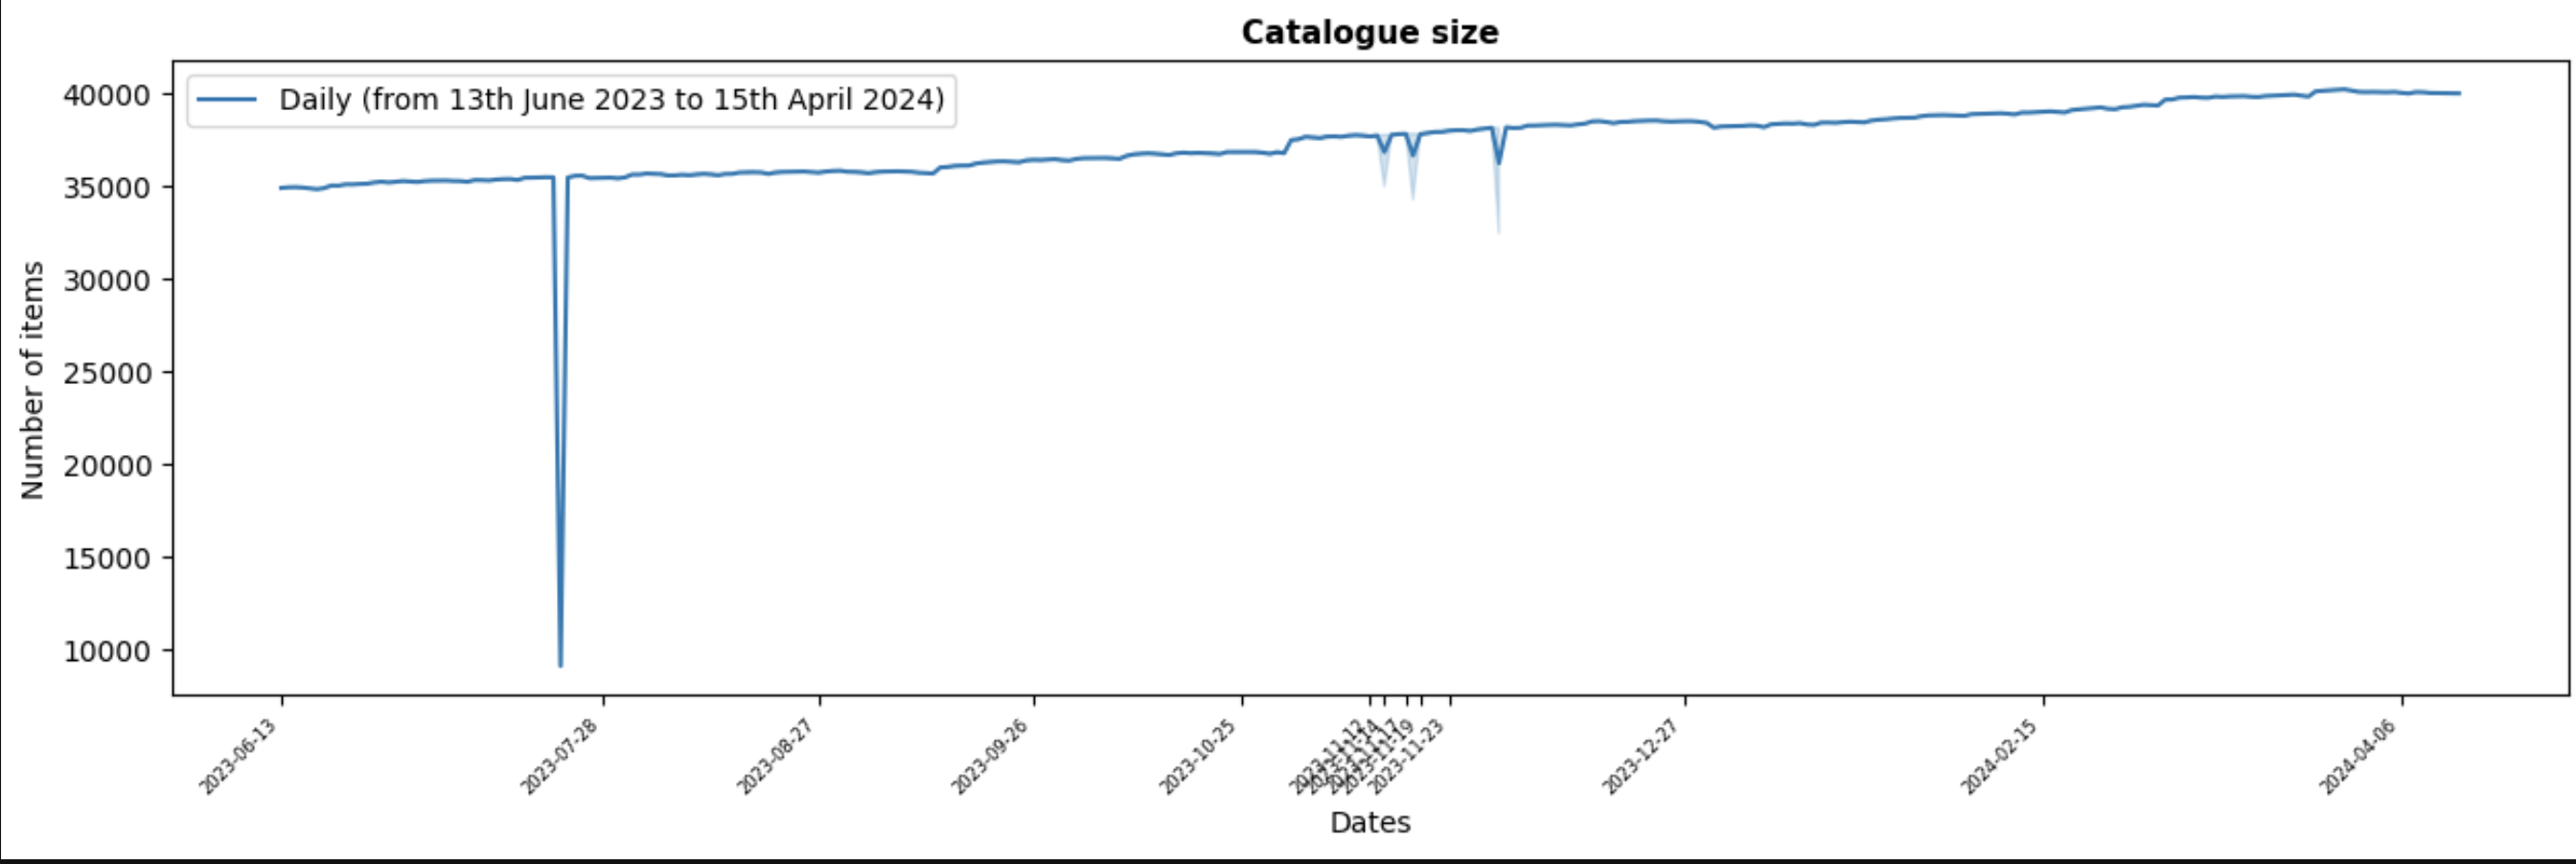
\includegraphics[scale=0.3]{catalogue_size}
  \caption{Daily catalogue size}
  \label{fig:catalogue_size}
\end{figure}

\begin{figure}[H]
  \centering
  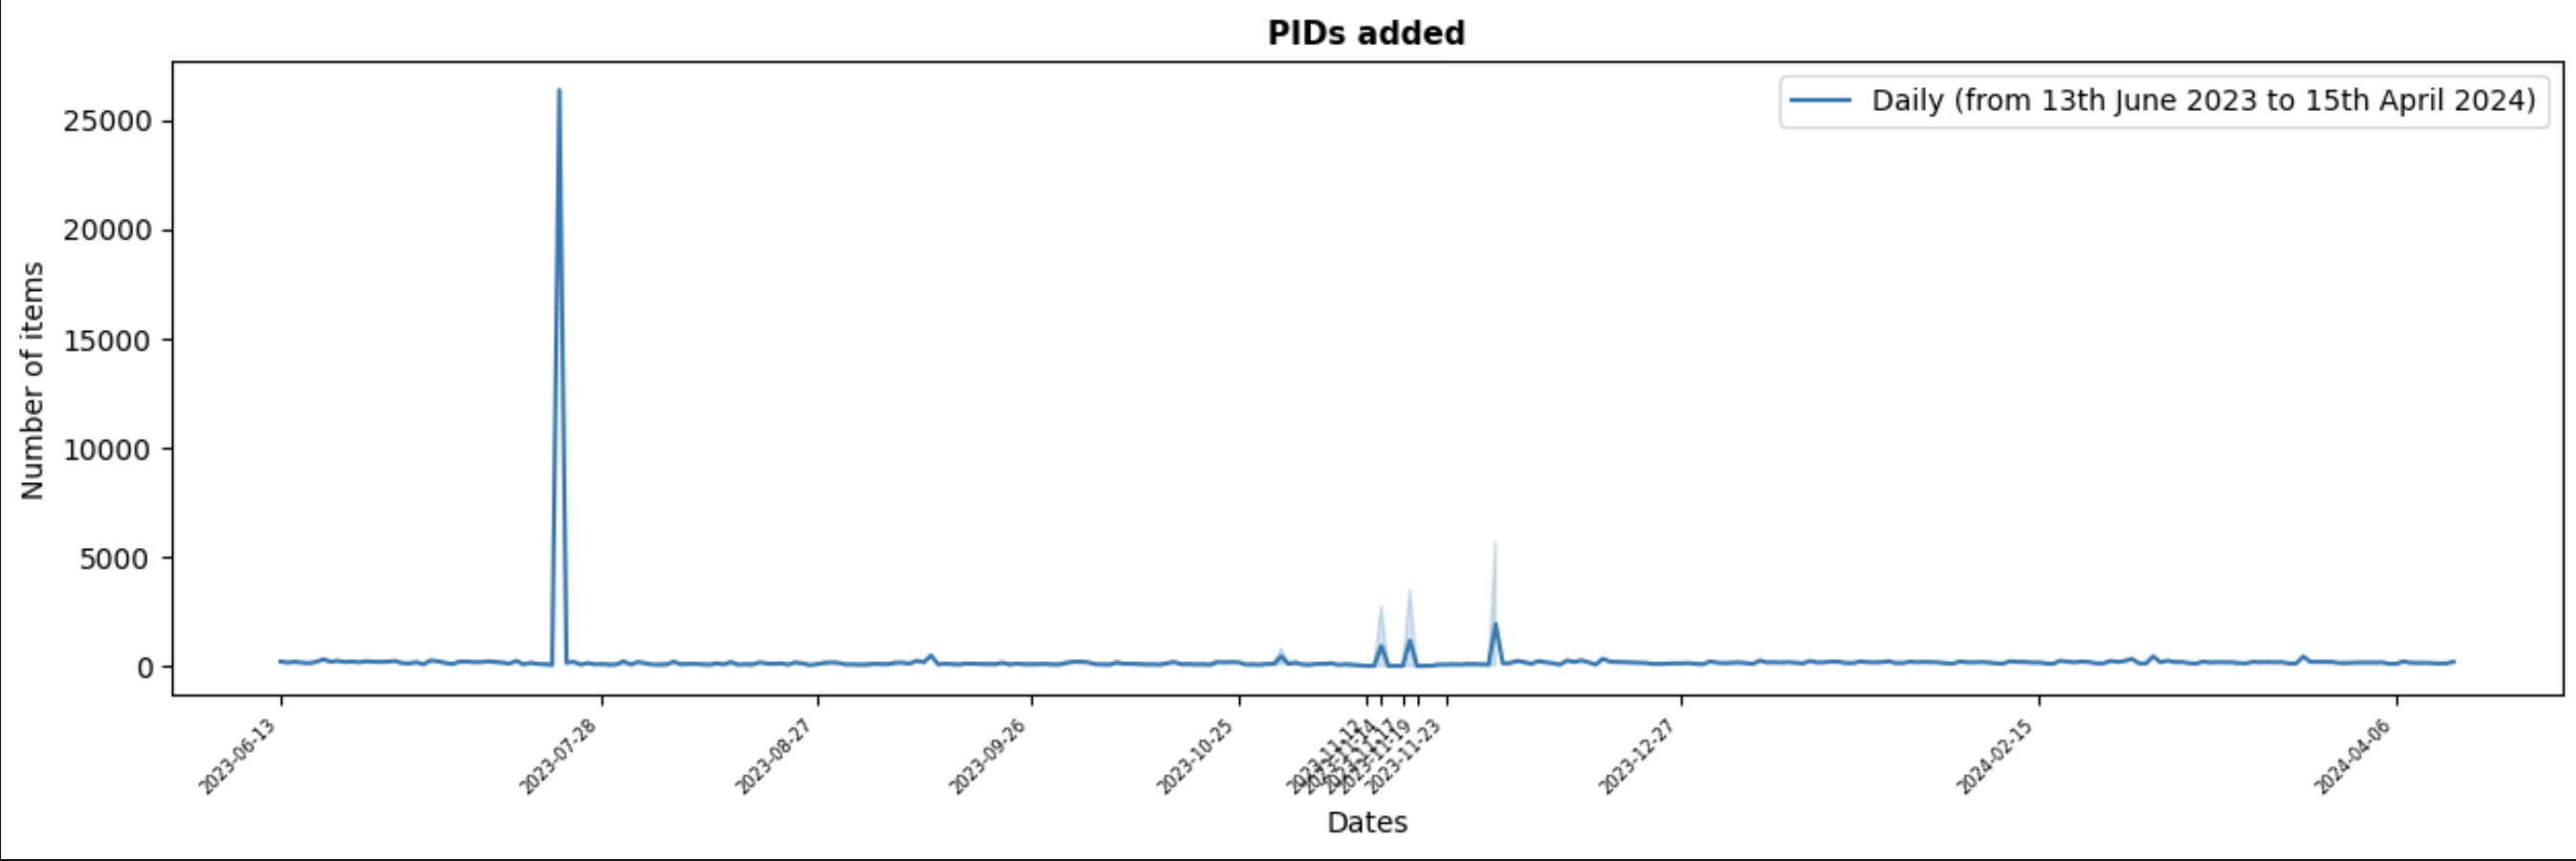
\includegraphics[scale=0.3]{catalogue_pids_added}
  \caption{Number of PIDs added daily}
  \label{fig:catalogue_pids_added}
\end{figure}

\begin{figure}[H]
  \centering
  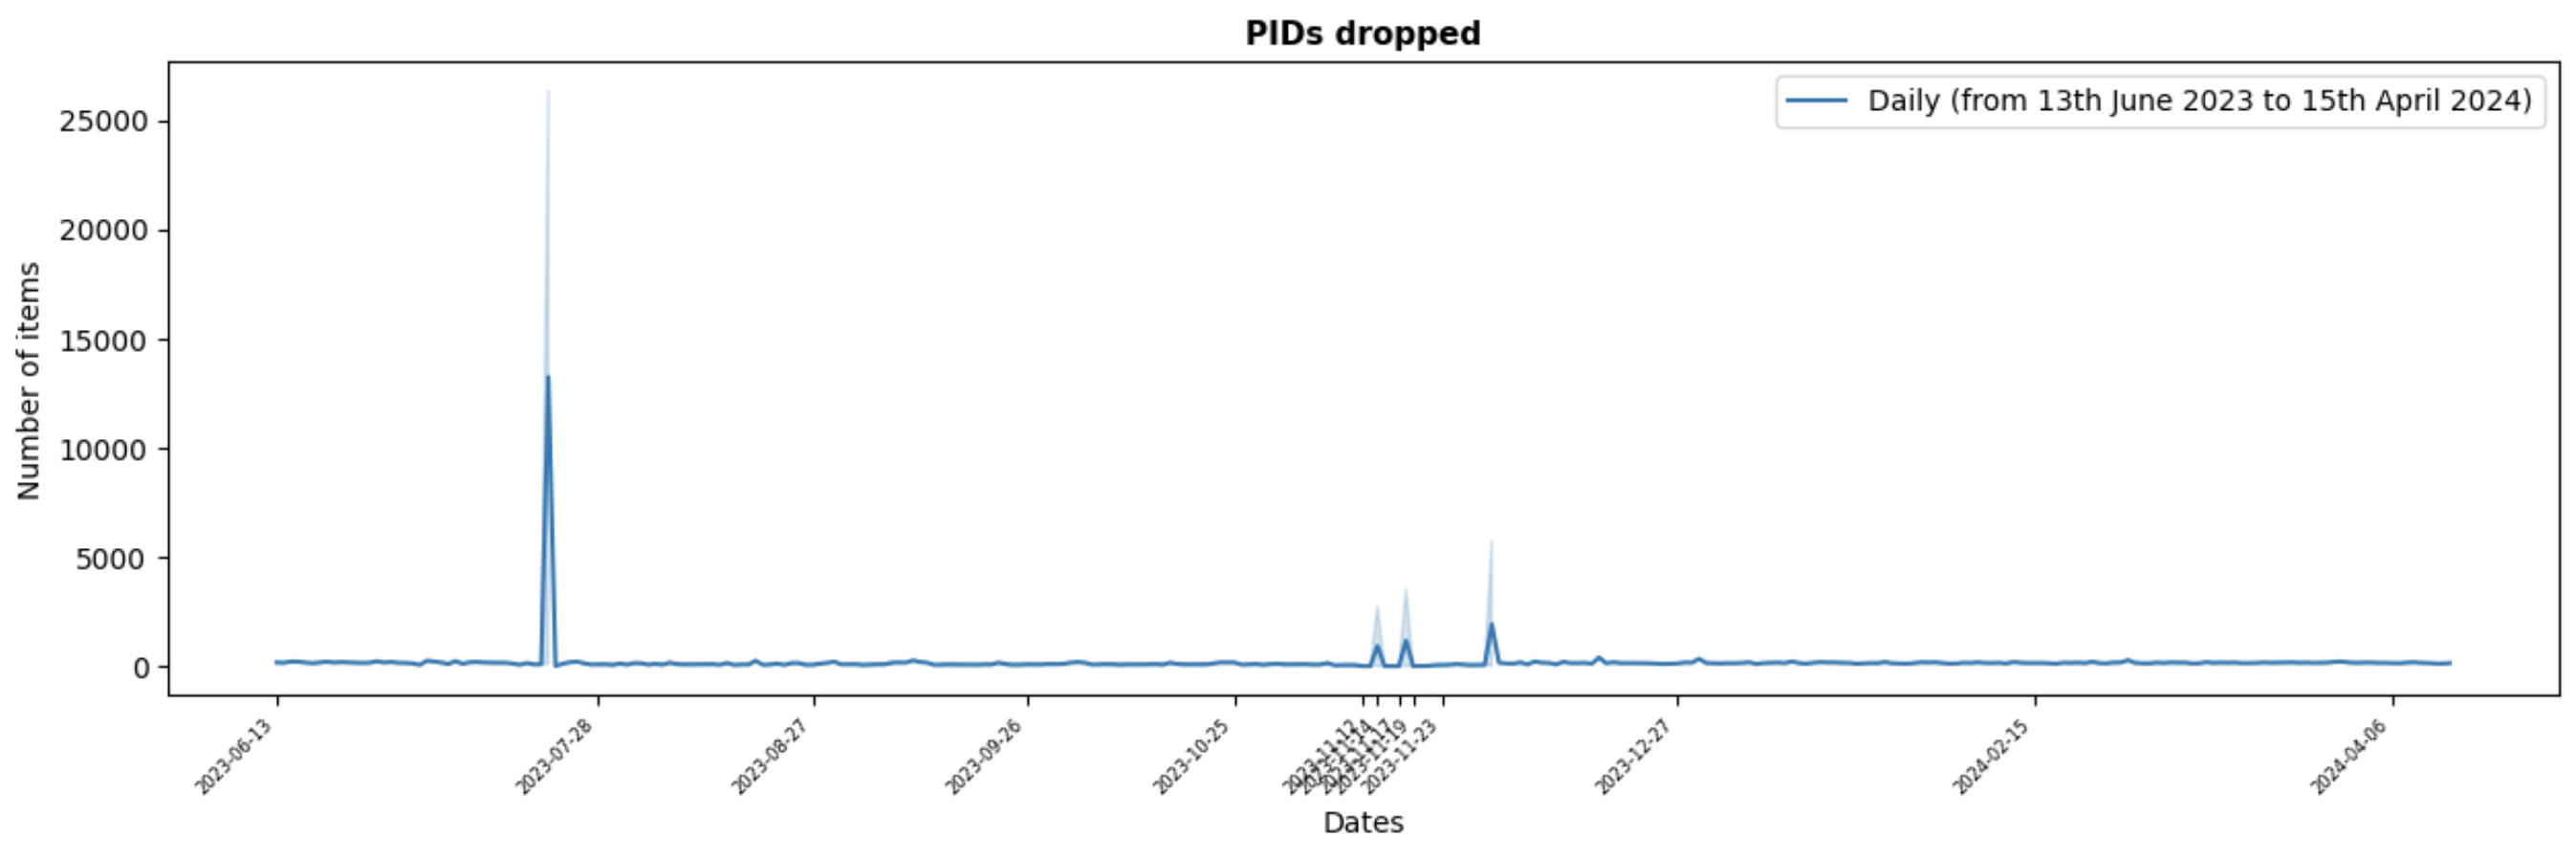
\includegraphics[scale=0.3]{catalogue_pids_dropped}
  \caption{Number of PIDs dropped daily}
  \label{fig:catalogue_pids_dropped}
\end{figure}

\begin{figure}[H]
  \centering
  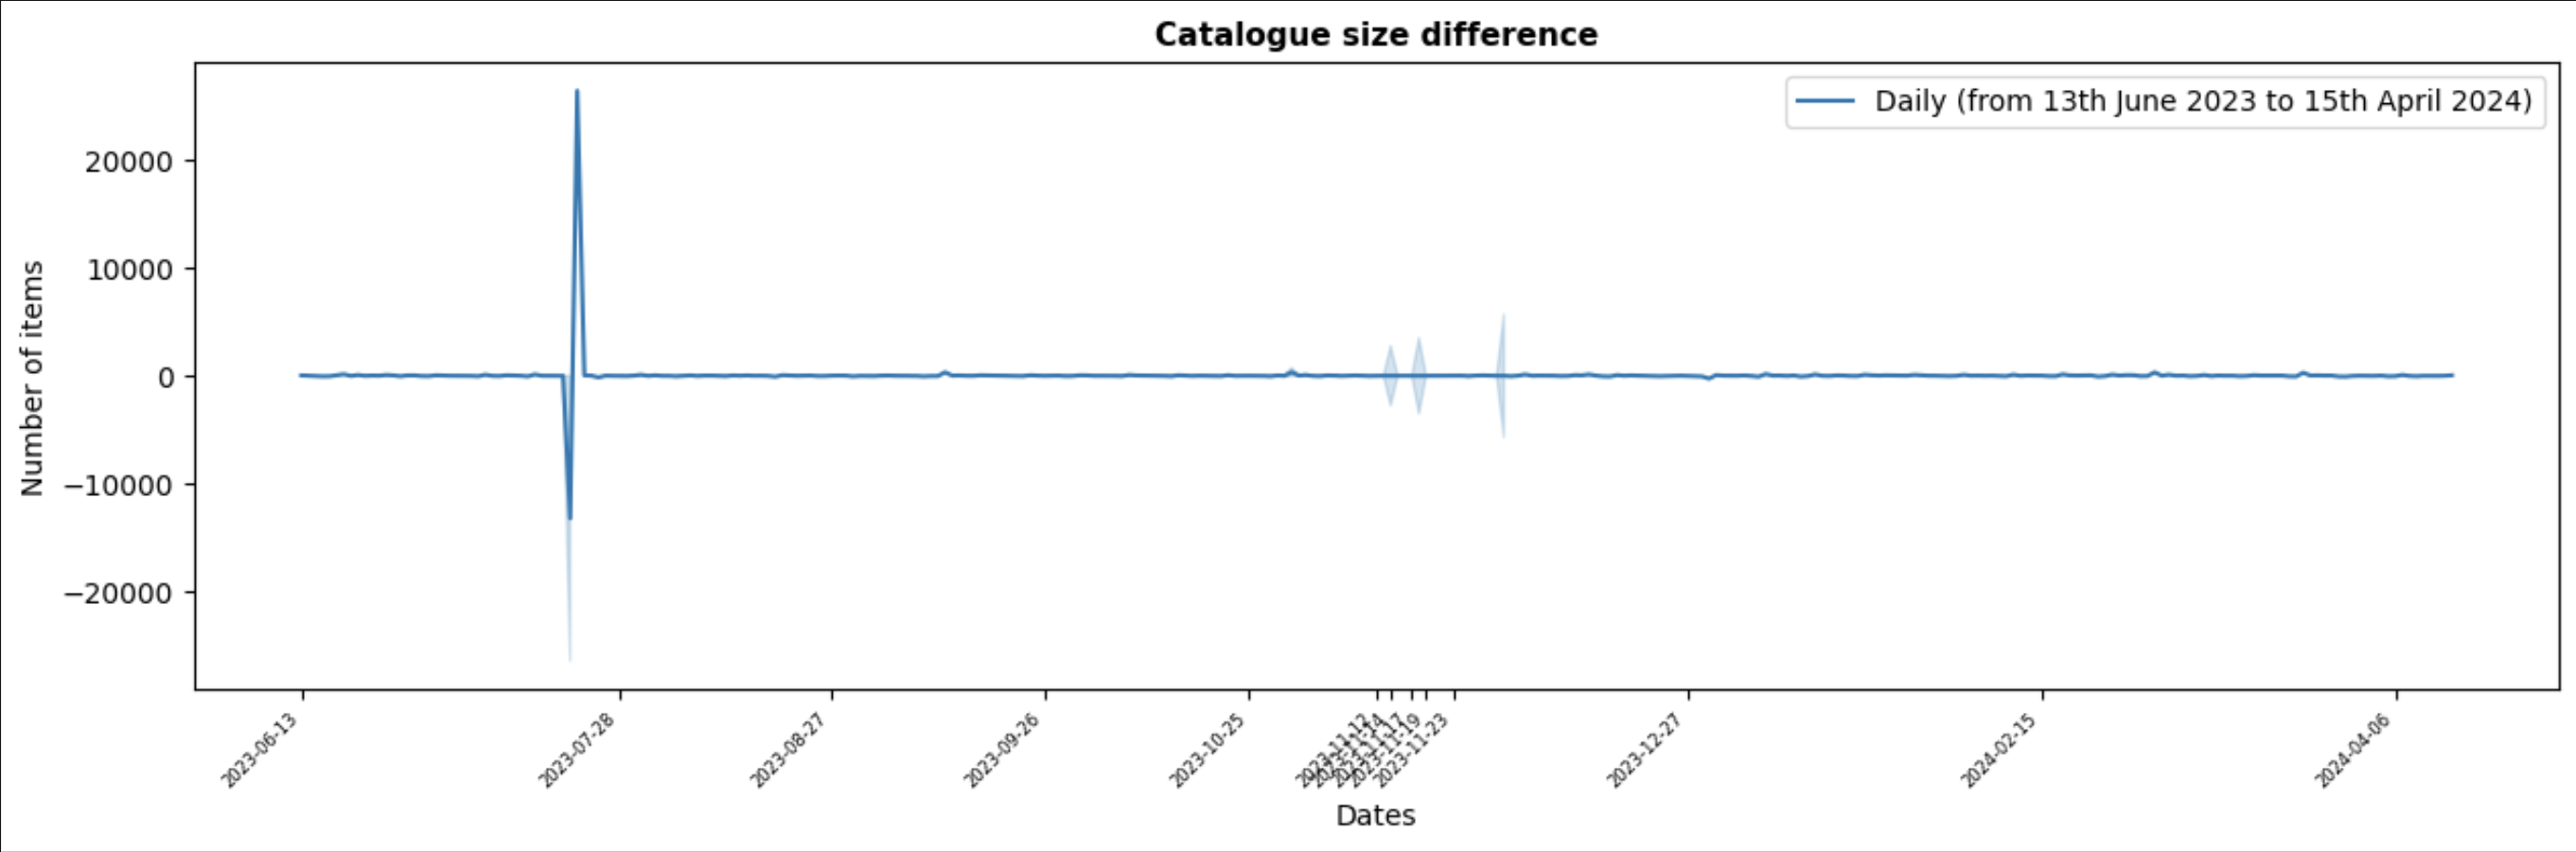
\includegraphics[scale=0.3]{catalogue_size_difference}
  \caption{Daily catalogue size difference}
  \label{fig:catalogue_size_diff}
\end{figure}

\begin{figure}[H]
  \centering
  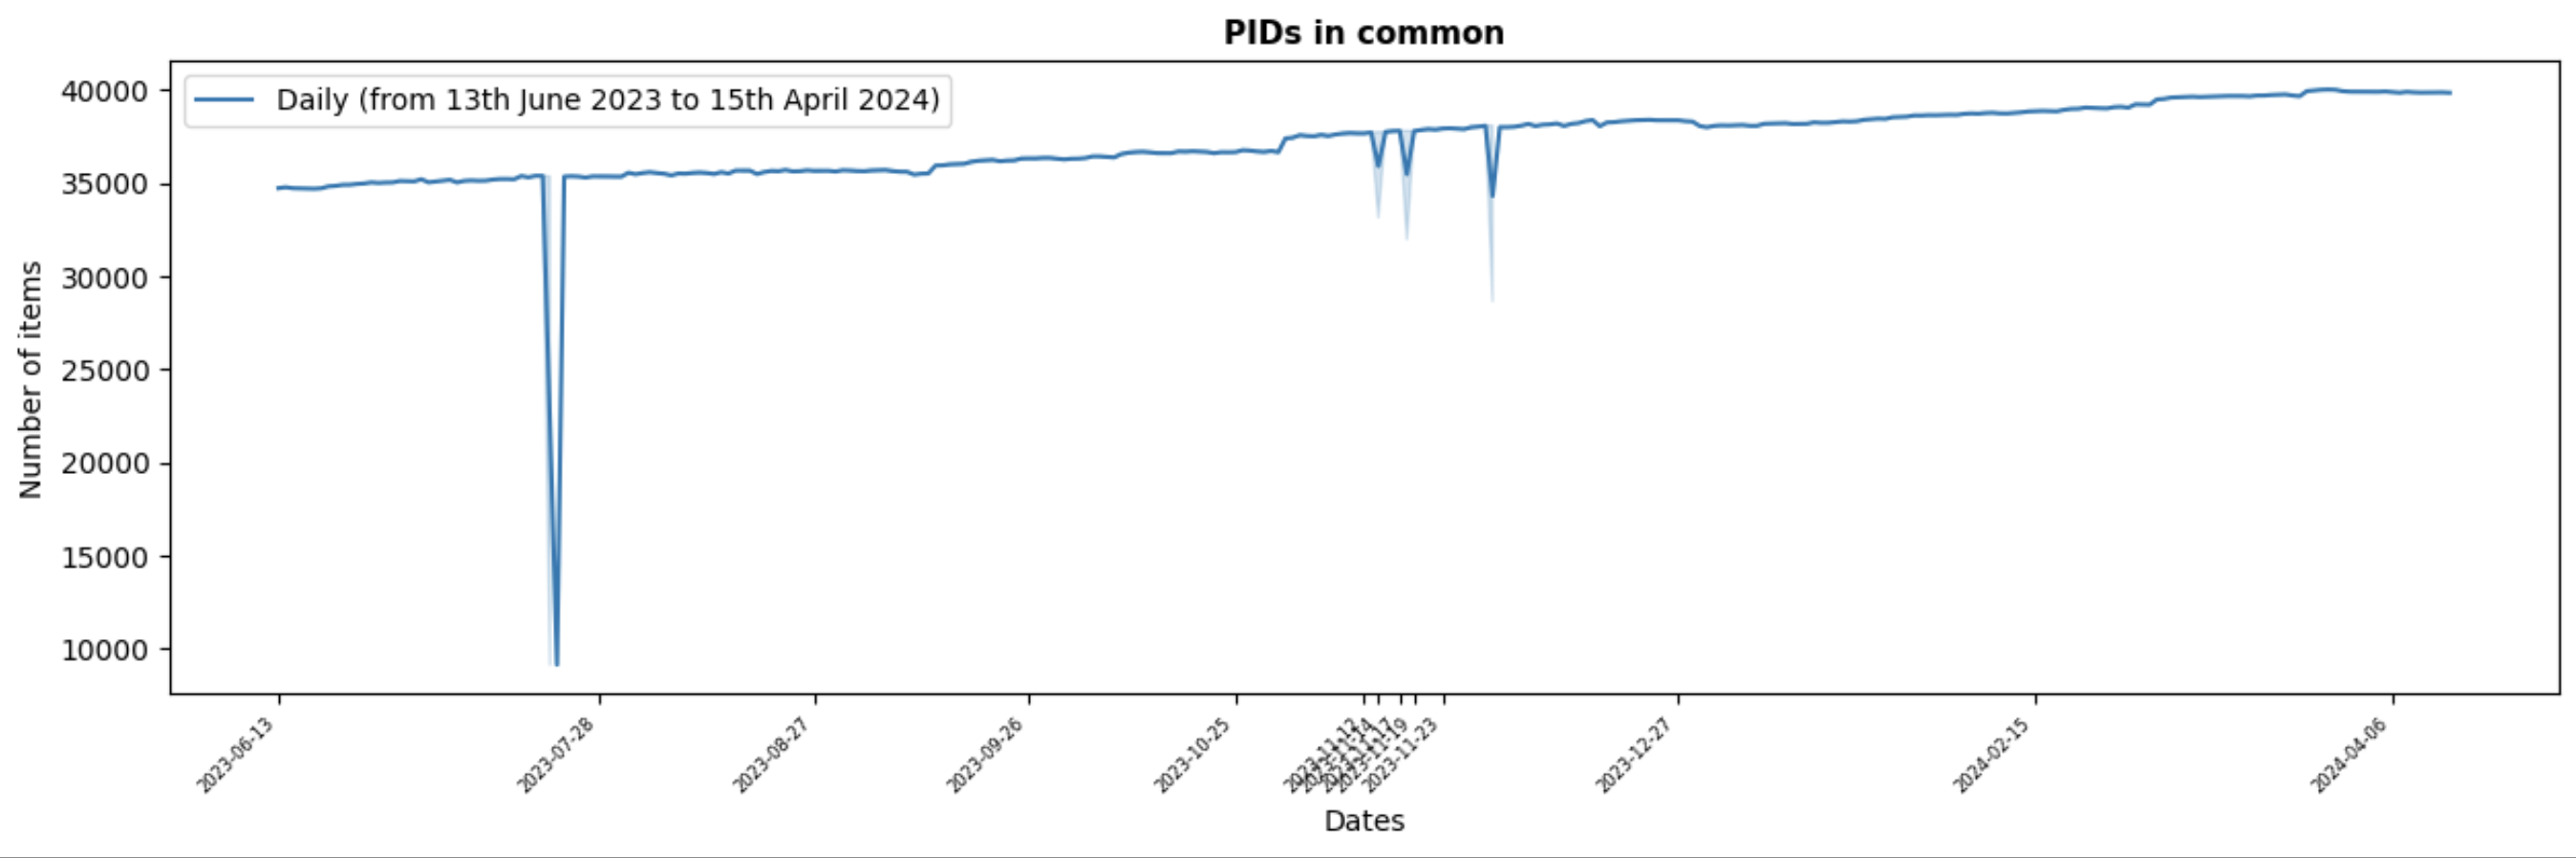
\includegraphics[scale=0.3]{catalogue_pids_common}
  \caption{Number of PIDs in common daily}
  \label{fig:catalogue_pids_common}
\end{figure}

\subsubsection{Programme structure and data distribution}

The \verb|18.19%| of programmes have a \textit{brand-episode} structure.
An example is the ``Christmas Celebration'' show, presented by Sally Magnusson.

\begin{figure}[H]
  \centering
  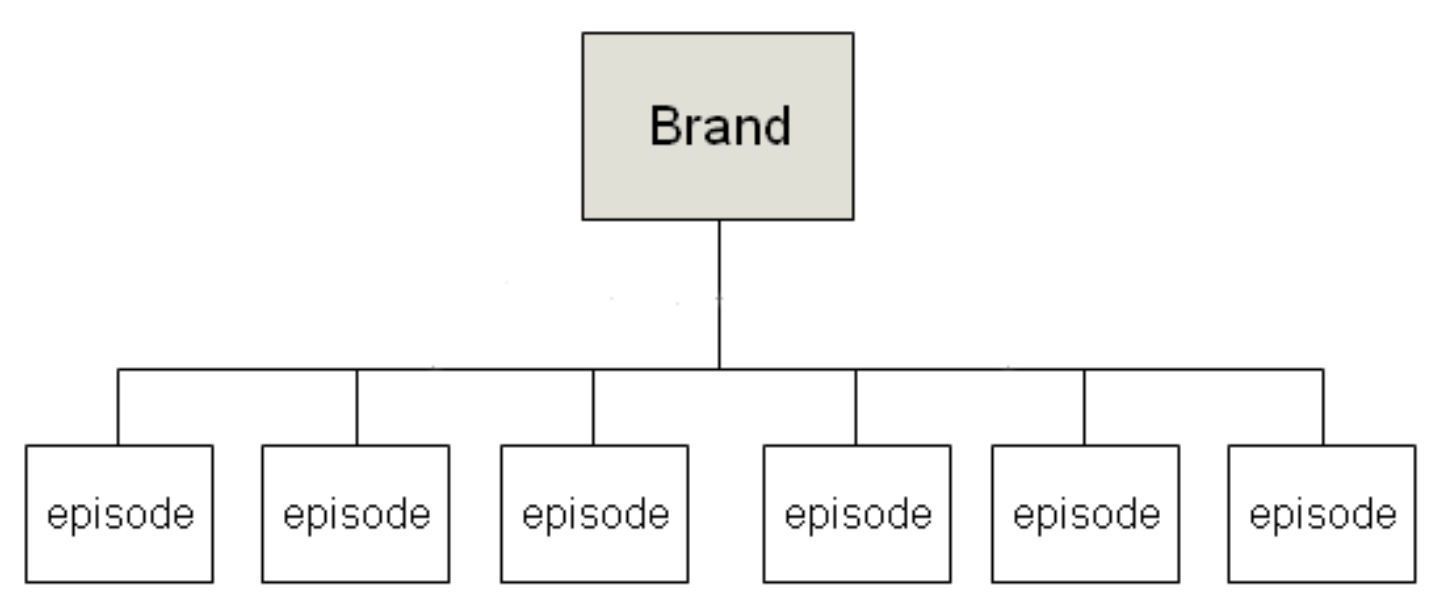
\includegraphics[scale=0.5]{pips_brand}
  \caption{PIP Brand-Episode hierarchy}
  \label{fig:pips_brand}
\end{figure}

The \verb|3.25%| of programmes have a Series-Episode structure.
An example is the four-part series ``Inside Obama's White House''.

\begin{figure}[H]
  \centering
  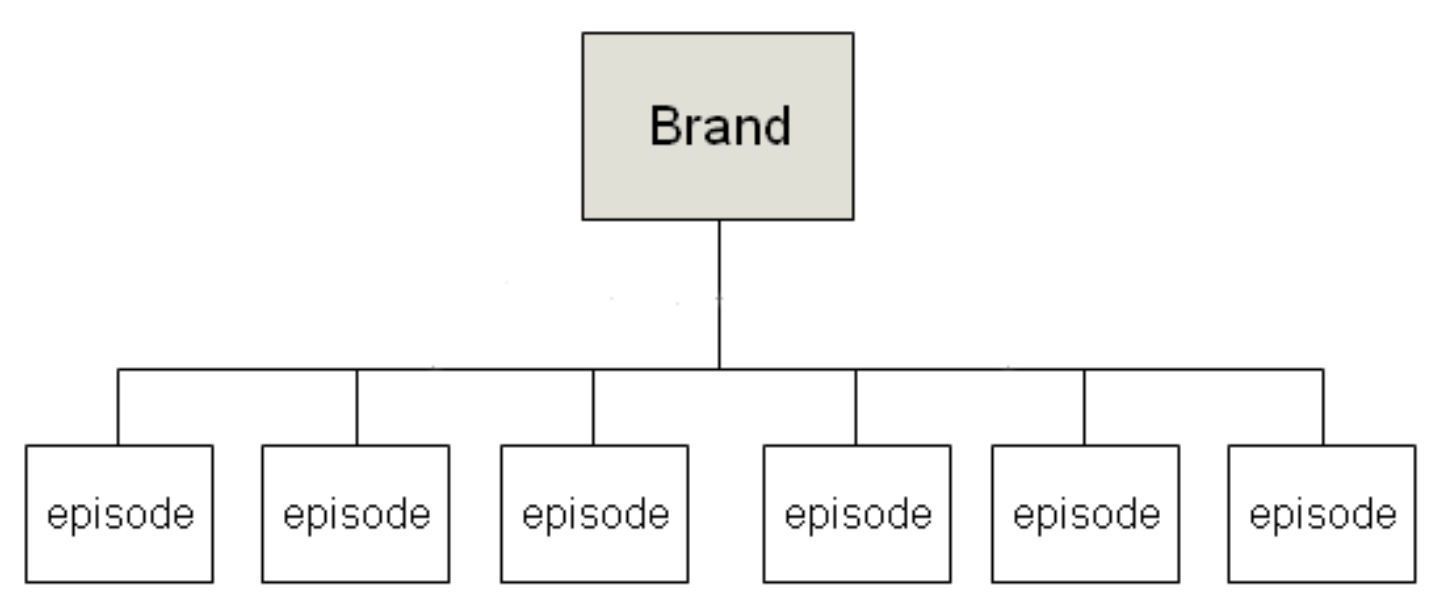
\includegraphics[scale=0.5]{pips_brand}
  \caption{PIP Brand-Episode hierarchy}
  \label{fig:pips_brand}
\end{figure}

\begin{figure}[H]
  \centering
  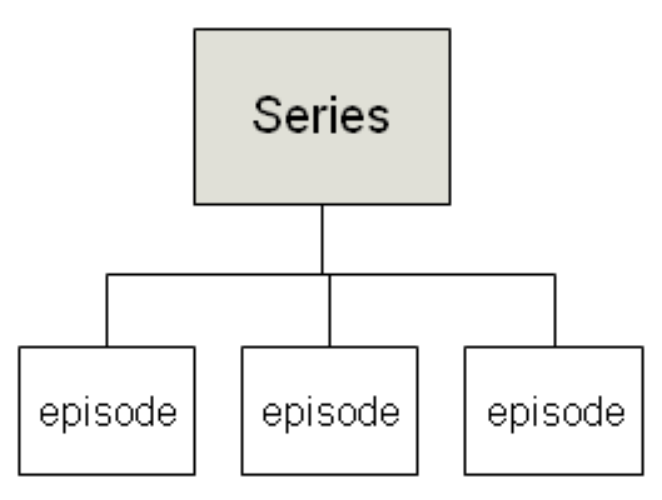
\includegraphics[scale=0.5]{pips_series}
  \caption{PIP Series-Episode hierarchy}
  \label{fig:pips_series}
\end{figure}

The \verb|75.12%| of programmes have a Brand-Series-Episode structure.
An example is the animated adventure comedy series ``Go Jetters''.

\begin{figure}[H]
  \centering
  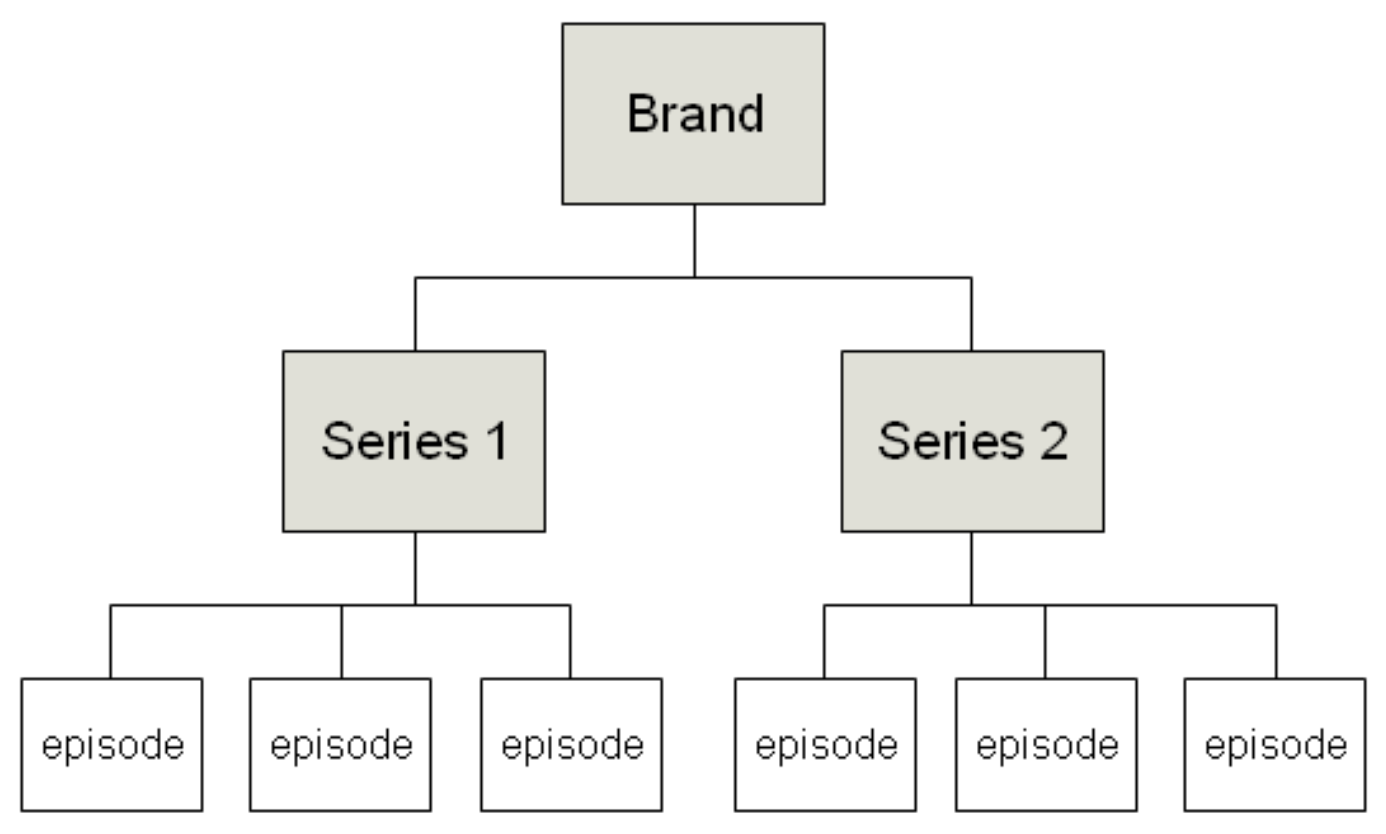
\includegraphics[scale=0.5]{pips_brand_series}
  \caption{PIP Brand-Series-Episode hierarchy}
  \label{fig:pips_brand_series}
\end{figure}

The remaining \verb|3.44%| of programmes are \textit{episode} only.
An example is the comedy documentary ``The Kemps: All Gold'' about the Spandau Ballet brother's lives.

\begin{figure}[H]
  \centering
  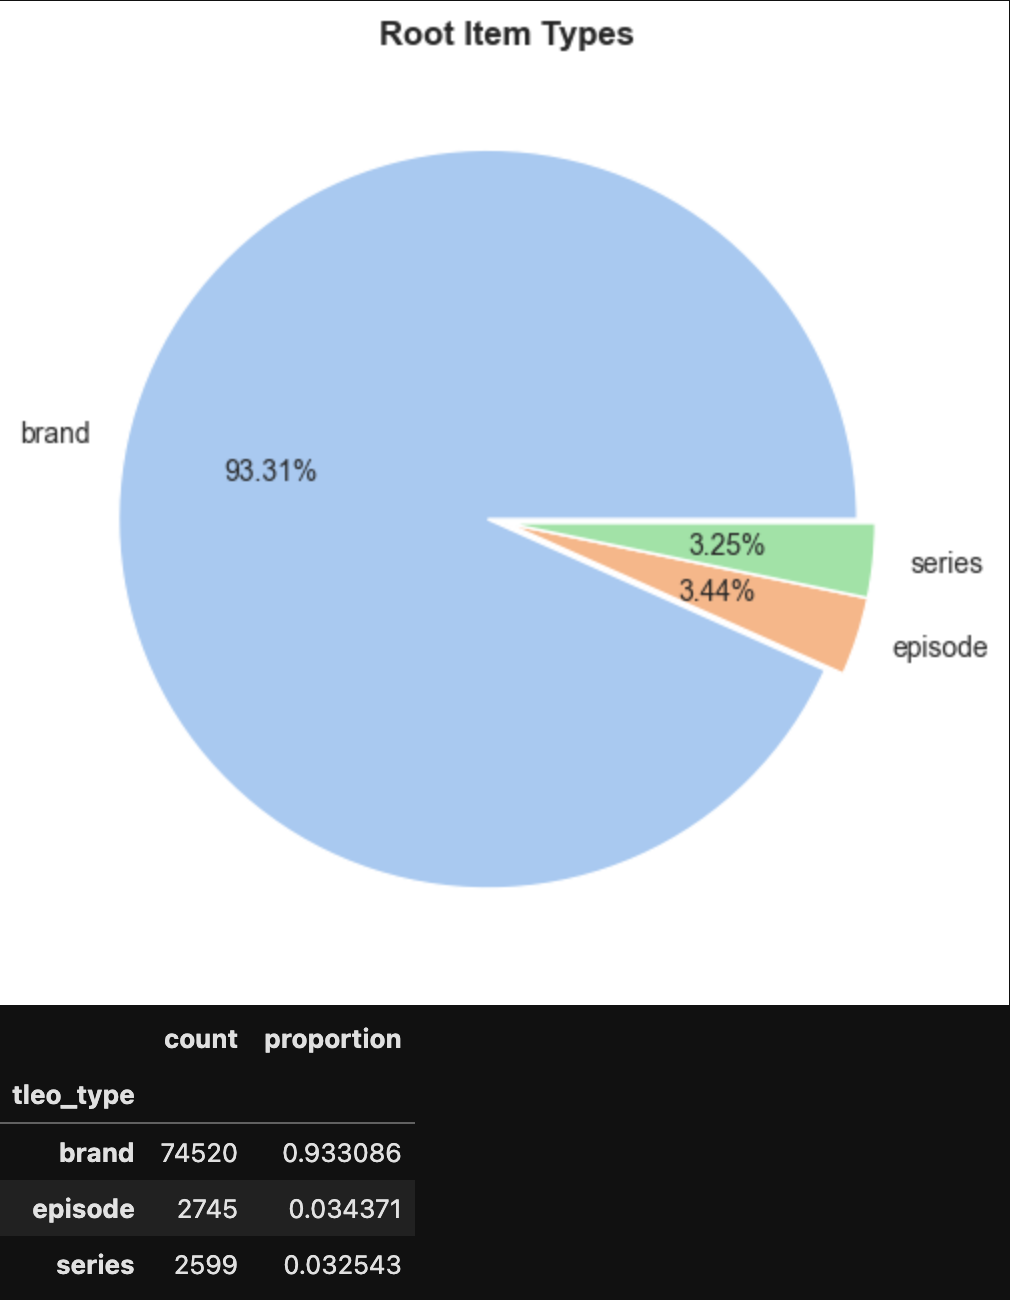
\includegraphics[scale=0.5]{programmes_root_item_types}
  \caption{Root item types distribution}
  \label{fig:programmes_root_item_types}
\end{figure}

\begin{figure}[H]
  \centering
  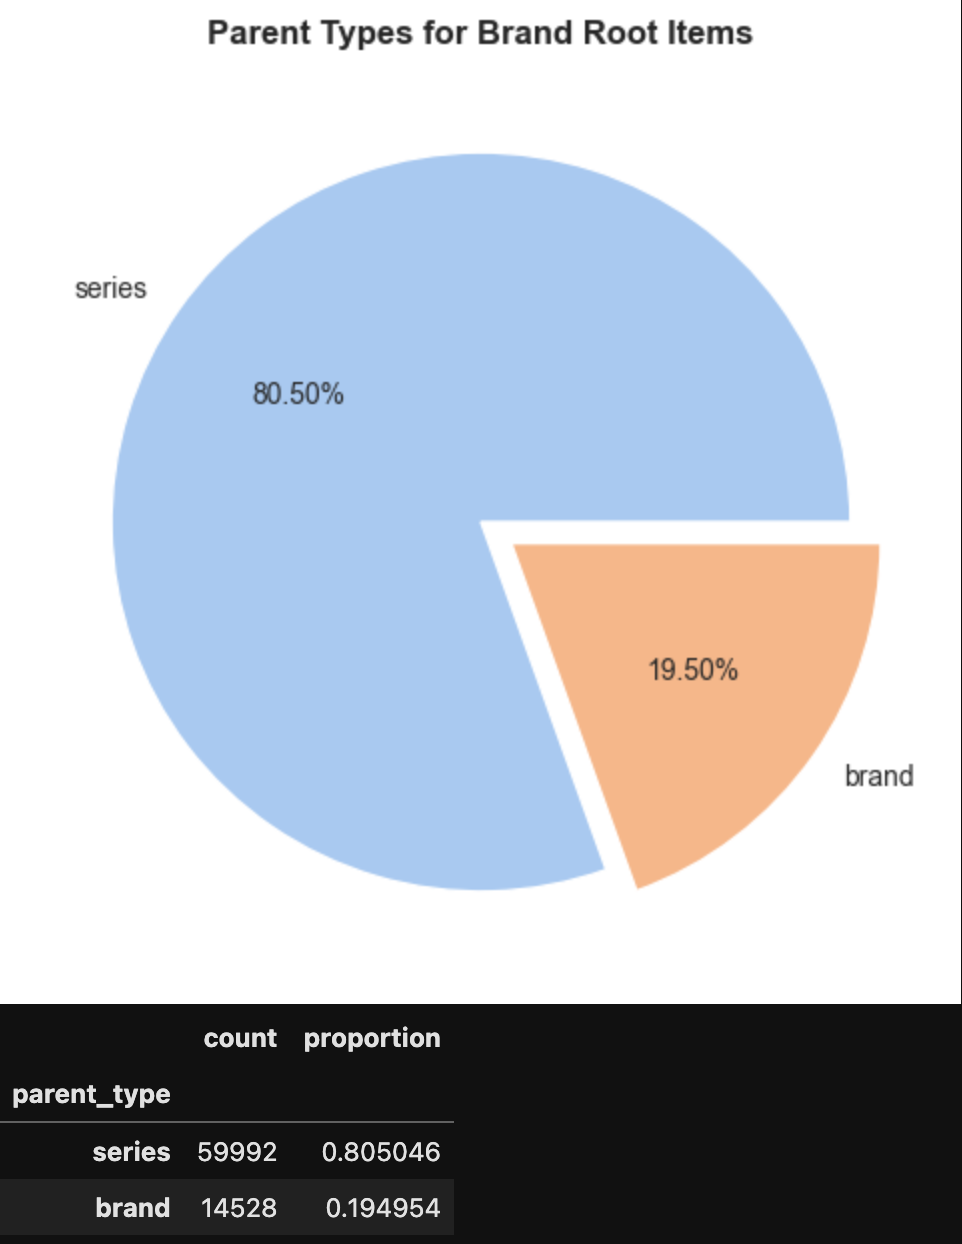
\includegraphics[scale=0.5]{programmes_parent_type.png}
  \caption{Parent types when the root item is a Brand}
  \label{fig:programmes_parent_type}
\end{figure}

\subsubsection{Recommendations}

\begin{figure}[H]
  \centering
  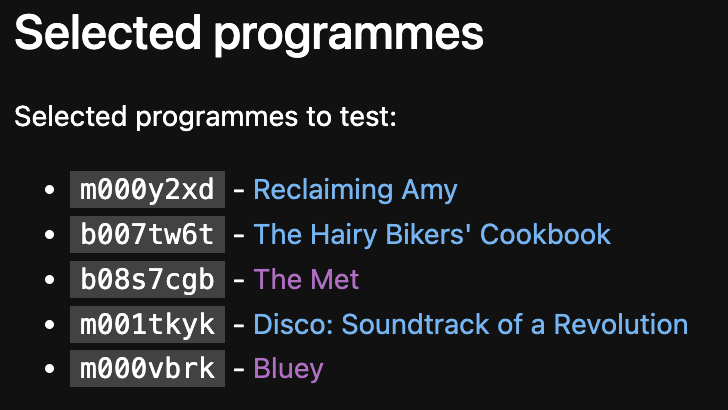
\includegraphics[scale=0.5]{selected_programmes}
  \caption{List of selected programmes for testing}
  \label{fig:selected_programmes}
\end{figure}

\begin{figure}[H]
  \centering
  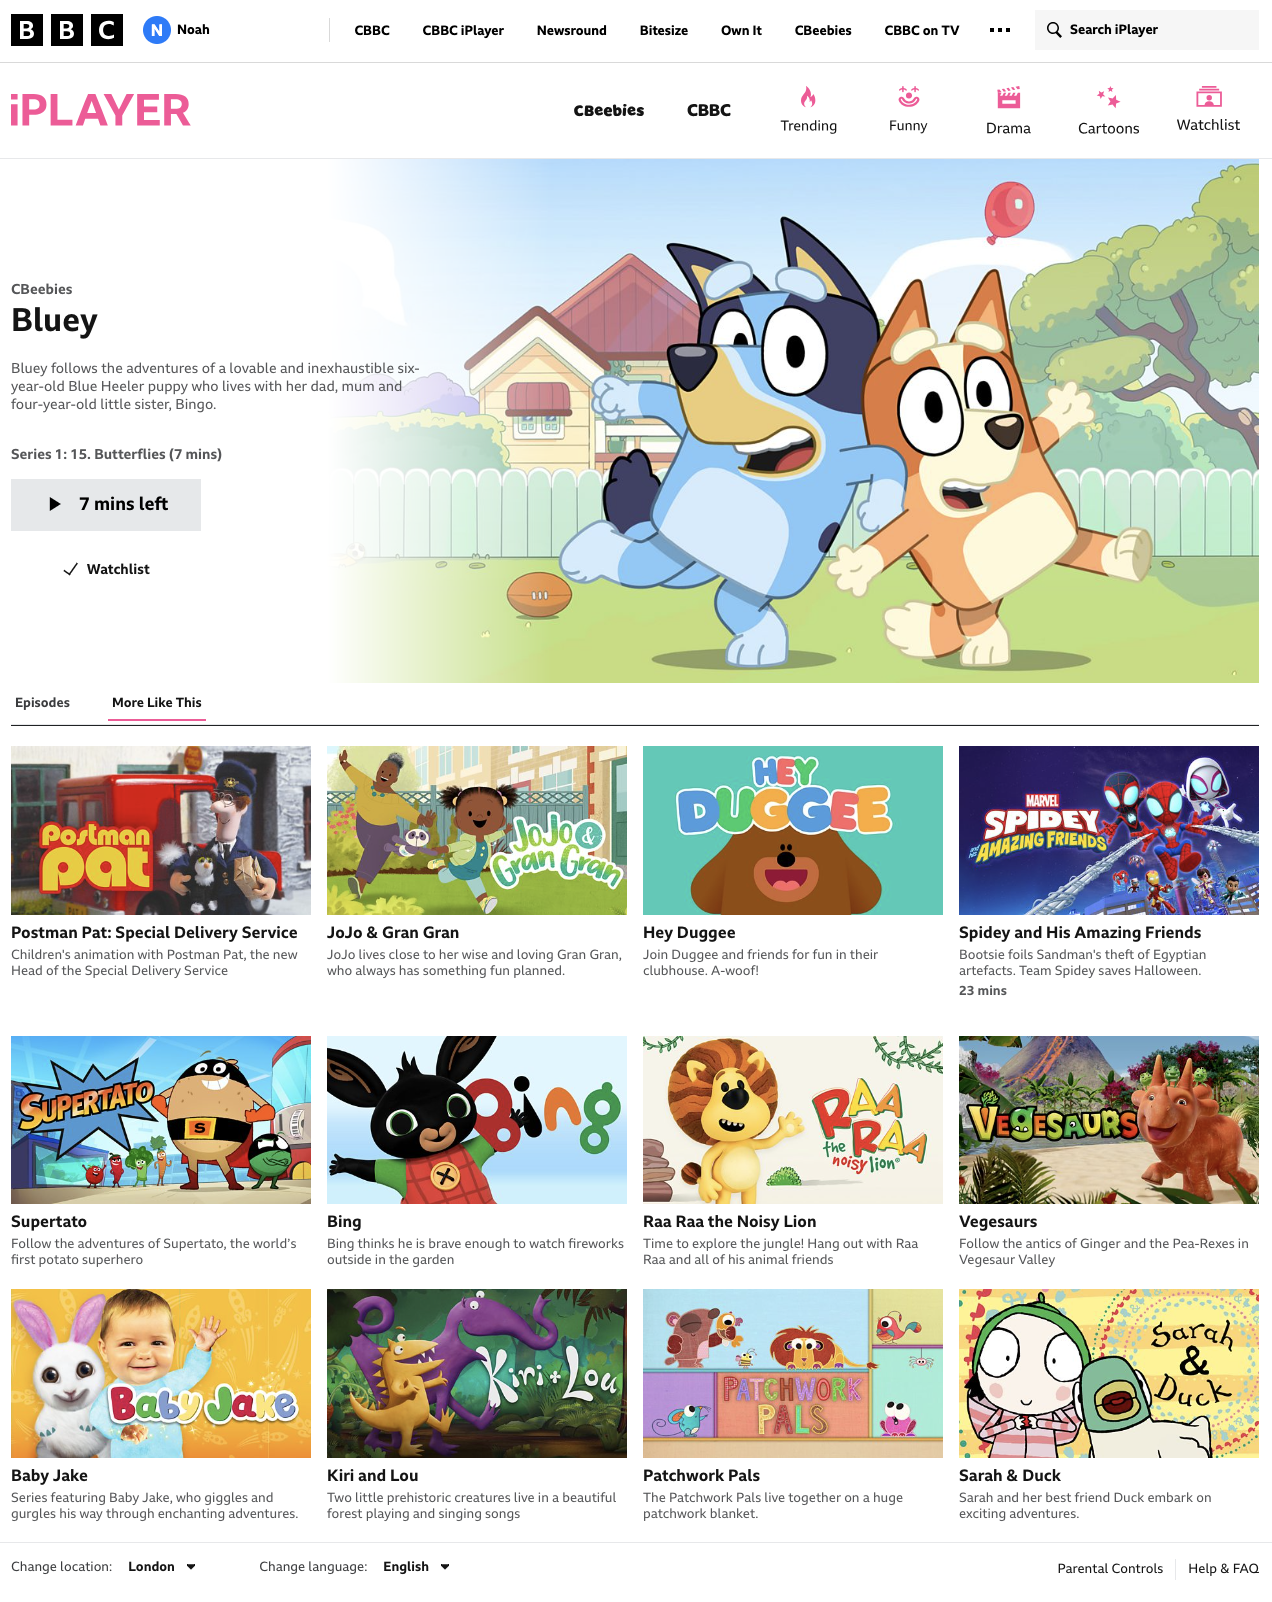
\includegraphics[scale=0.5]{bluey}
  \caption{The "More Like This" secton on BBC iPlayer}
  \label{fig:bluey}
\end{figure}

\begin{figure}[H]
  \centering
  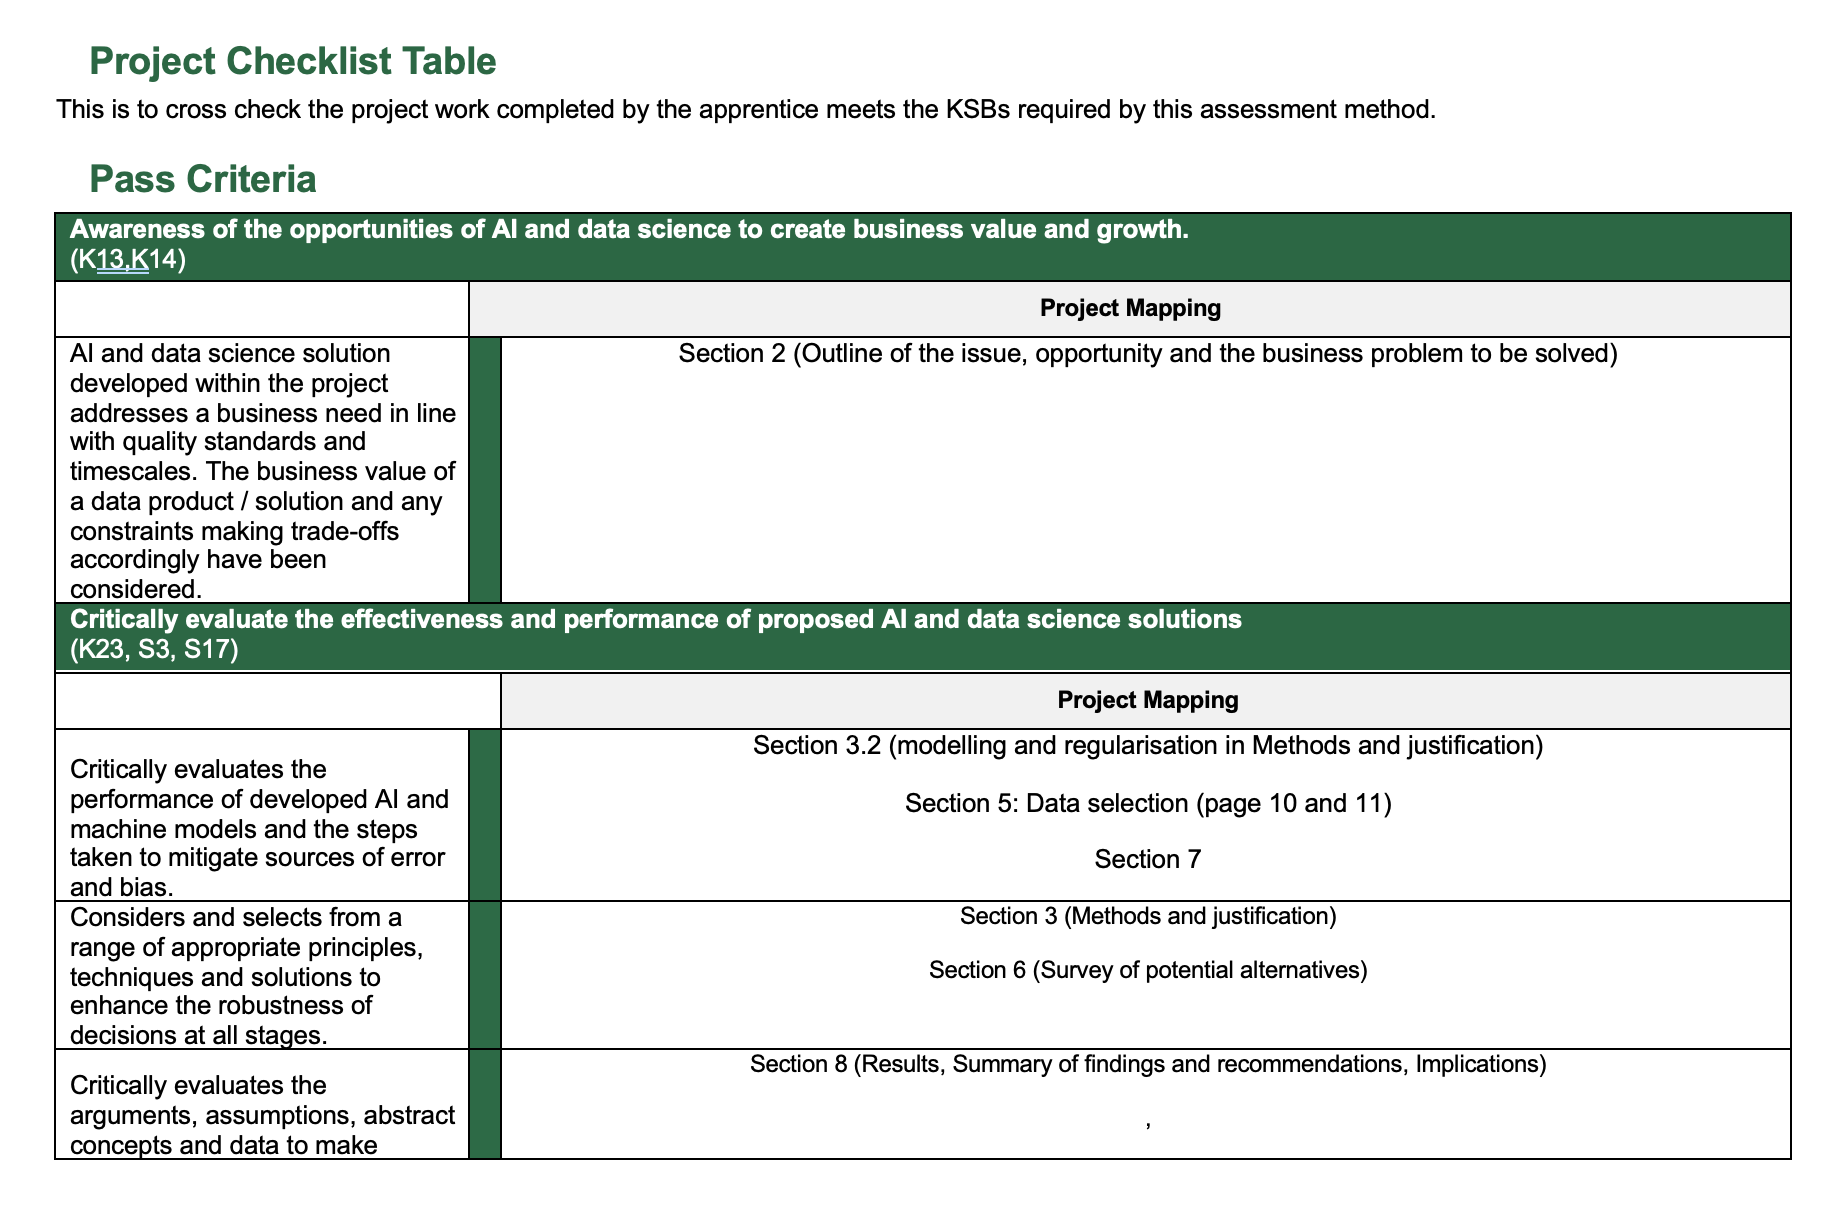
\includegraphics[scale=0.5]{recommendations/0}
  \caption{"Bluey" Programme Page on iPlayer}
  \label{fig:recommendations:0}
\end{figure}

\begin{figure}[H]
  \centering
  
\includegraphics[scale=0.5]{recommendations/1}
  \caption{"Patchwork Pals": 1st recommendation (similarity score 0.9602)}
  \label{fig:recommendations:1}
\end{figure}

\begin{figure}[H]
  \centering
  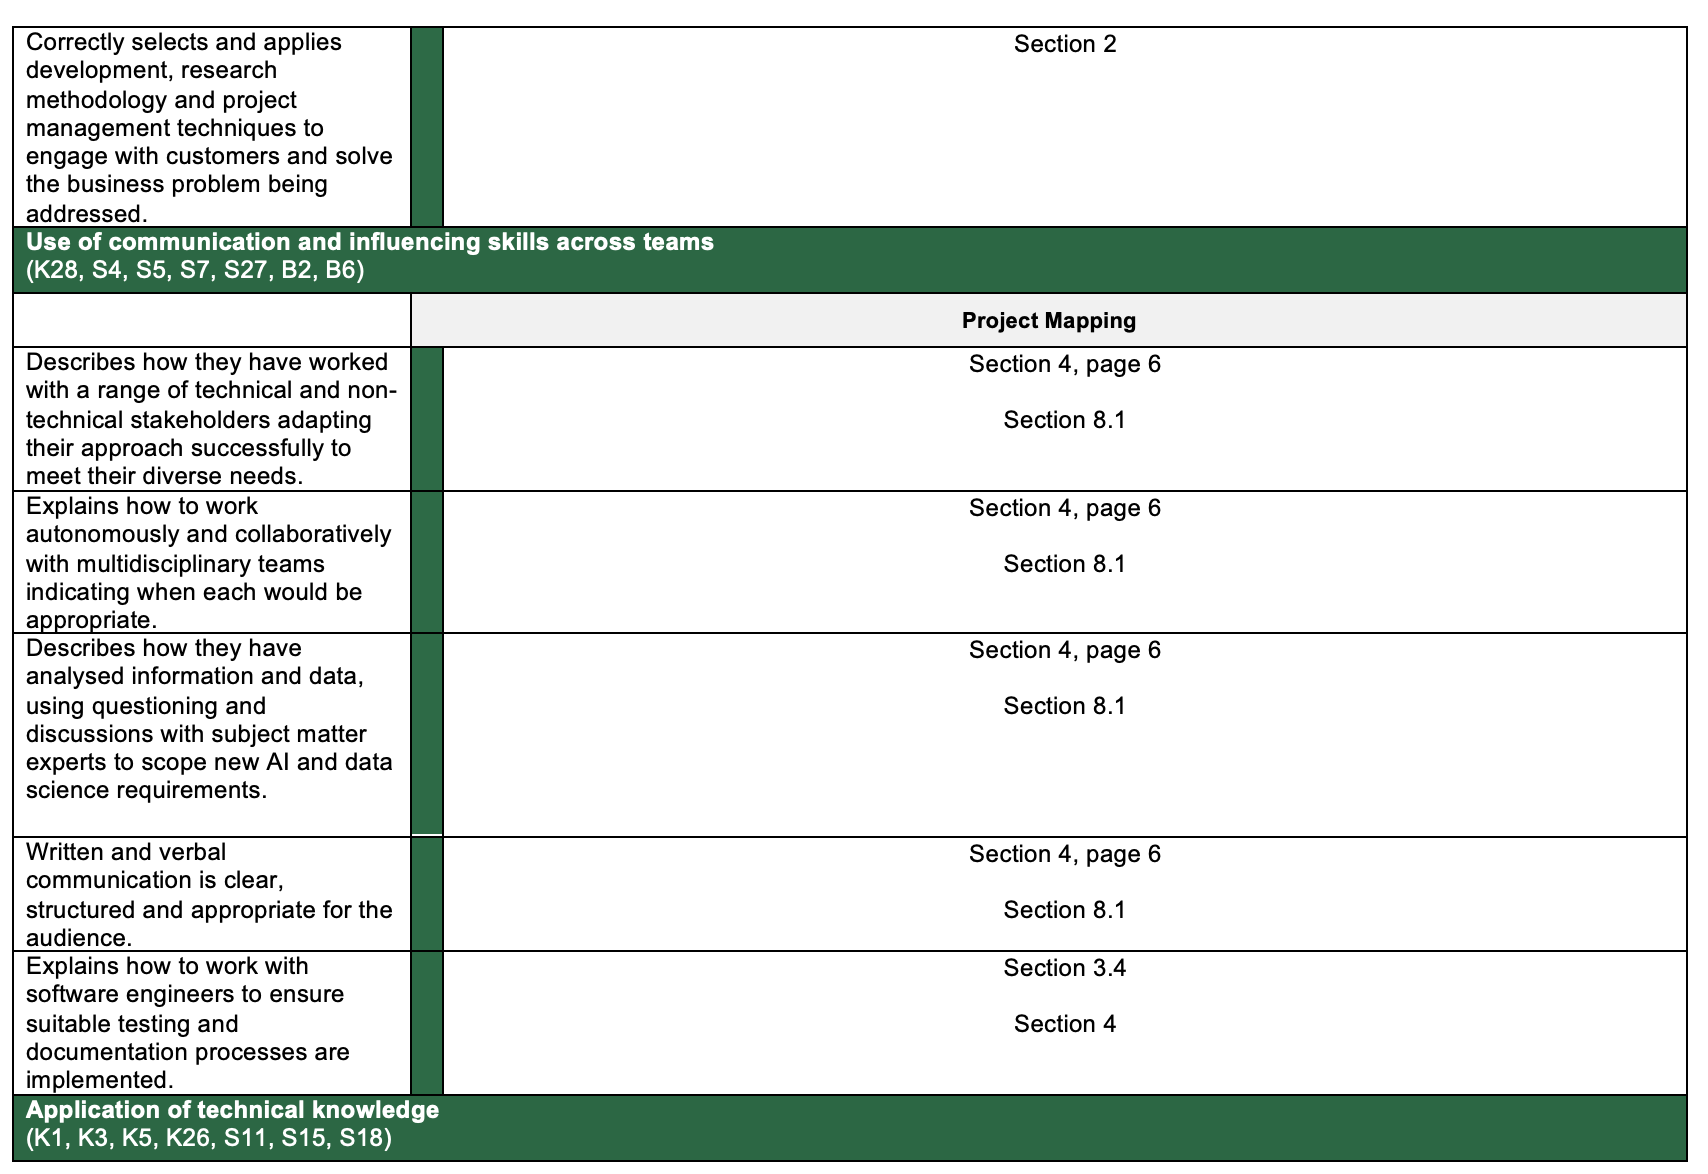
\includegraphics[scale=0.5]{recommendations/2}
  \caption{"Timmy Time": 2nd recommendation (similarity score 0.9474)}
  \label{fig:recommendations:1}
\end{figure}

\begin{figure}[H]
  \centering
  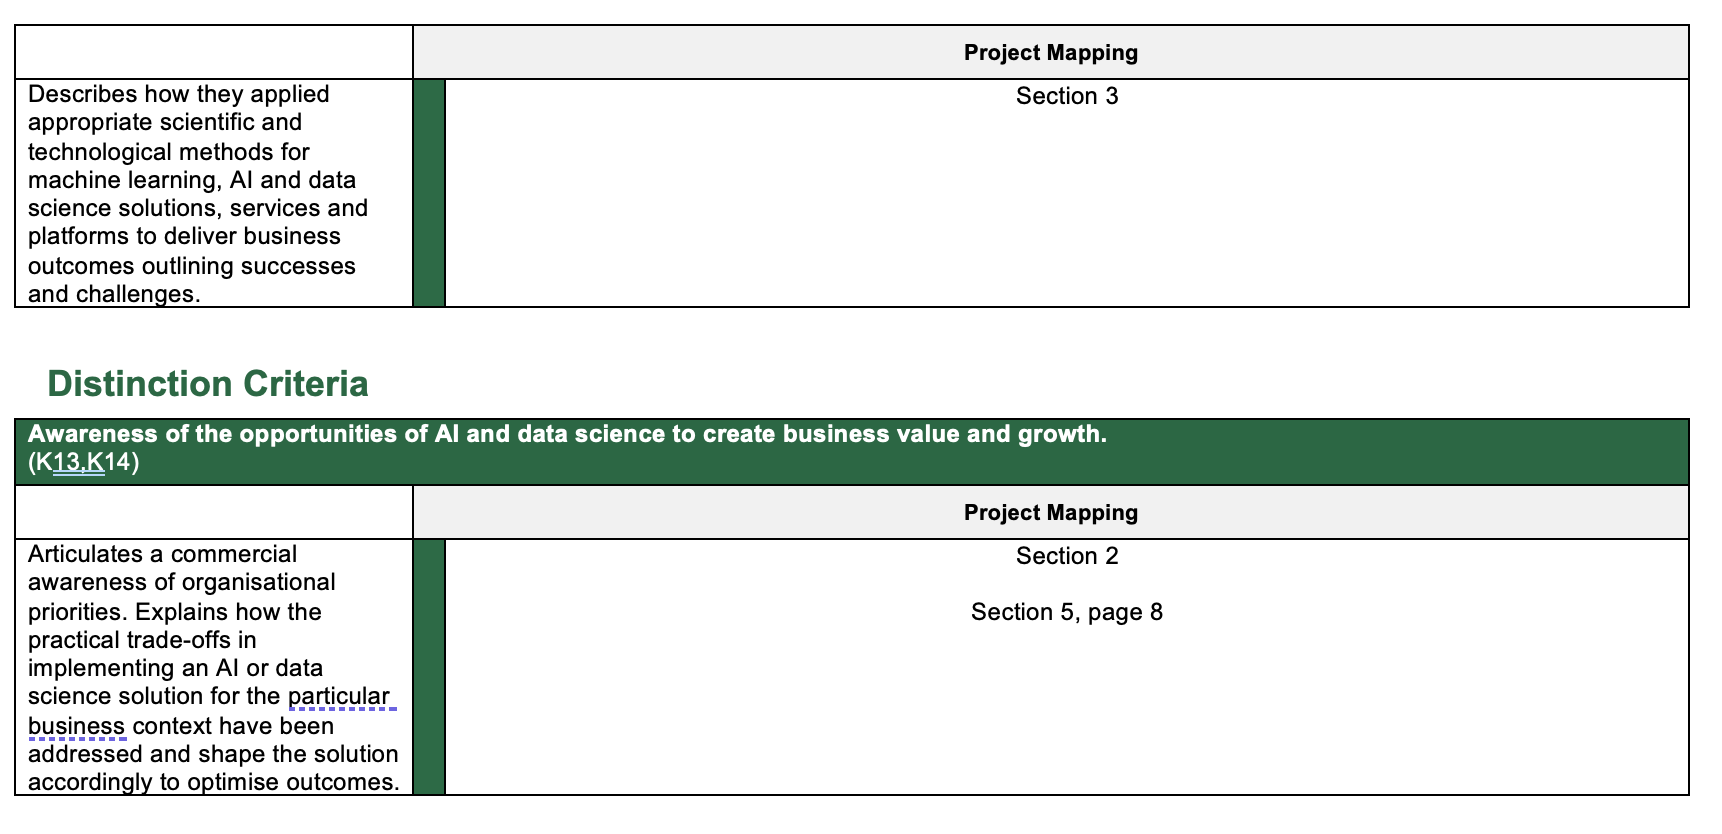
\includegraphics[scale=0.5]{recommendations/3}
  \caption{"Fireman Sam": 3rd recommendation (similarity score 0.9420)}
  \label{fig:recommendations:1}
\end{figure}

\begin{figure}[H]
  \centering
  
\includegraphics[scale=0.5]{recommendations/4}
  \caption{"Arthur": 4th recommendation (similarity score 0.9406)}
  \label{fig:recommendations:1}
\end{figure}

% This is highly recommended
% The level of detail needed is section headings and page numbers illustrating where the criteria have been met
\subsection{Mapping of the project report to the pass criteria}
